\newpage
\subsection{How do solar cells absorb light?}
In this section we are going to learn how a solar cells interact with light.  Firstly, let's have a look at the solar spectrum.  Sunlight contains many wavelengths of light, from ultraviolet light, though to visible light to infrared.  The human eye can only see a small fraction of the light emitted by the sun.  OghmaNano stores a copy of the suns spectrum to perform the simulations.  Let's have a look at this spectrum, to do this go to the \emph{Database} tab, the choose \emph{Optical database}.  This should, bring up a window as shown in figure \ref{fig:optical_database}

\begin{figure}[h!]
\centering
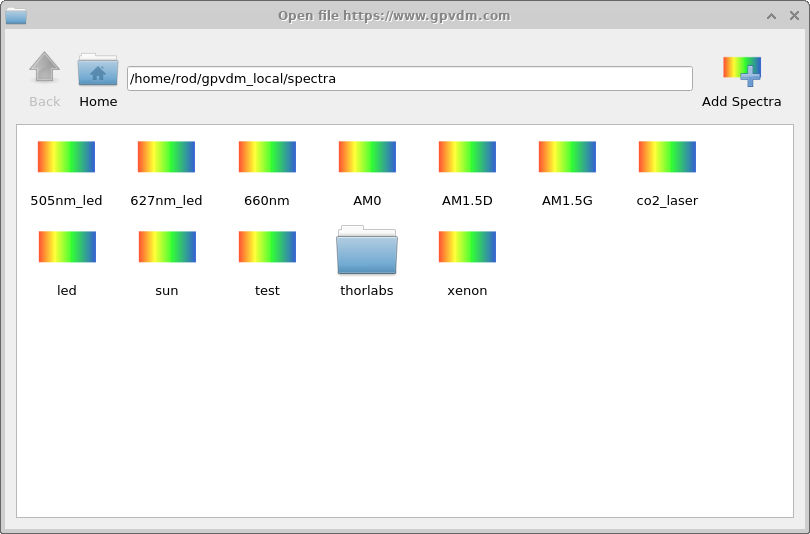
\includegraphics[width=0.6\textwidth]{./images/running/optical_database.png}
\caption{The optical database viewer}
\label{fig:optical_database}
\end{figure}

Double click on the icon called, \emph{AM1.5G}, this should bring up a spectrum of the sun's spectrum.  Have a look at where the peak of the spectrum is.  Now close this window, and open the spectrum called $led$.  Where is the peak of this spectrum.


\begin{figure}[H]
\centering
\begin{tabular}{ c c }

\raisebox{-.1\height}{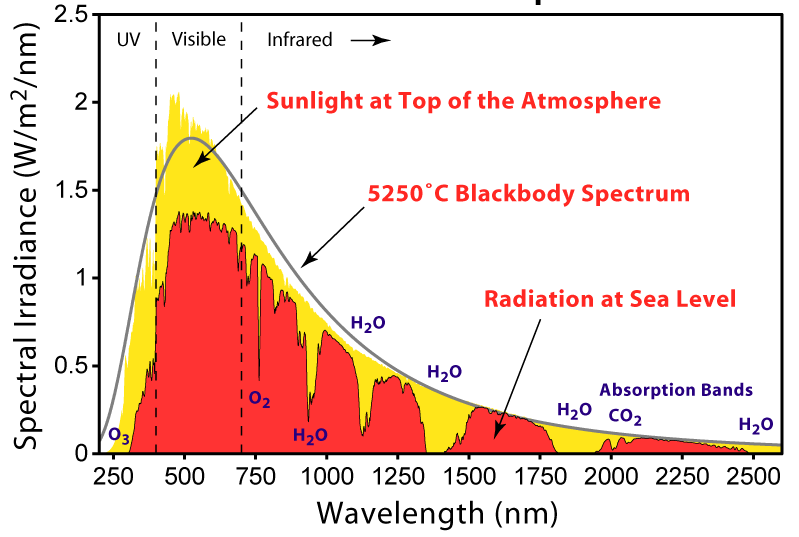
\includegraphics[width=0.45\textwidth]{./images/running/spectrum.png}}

&
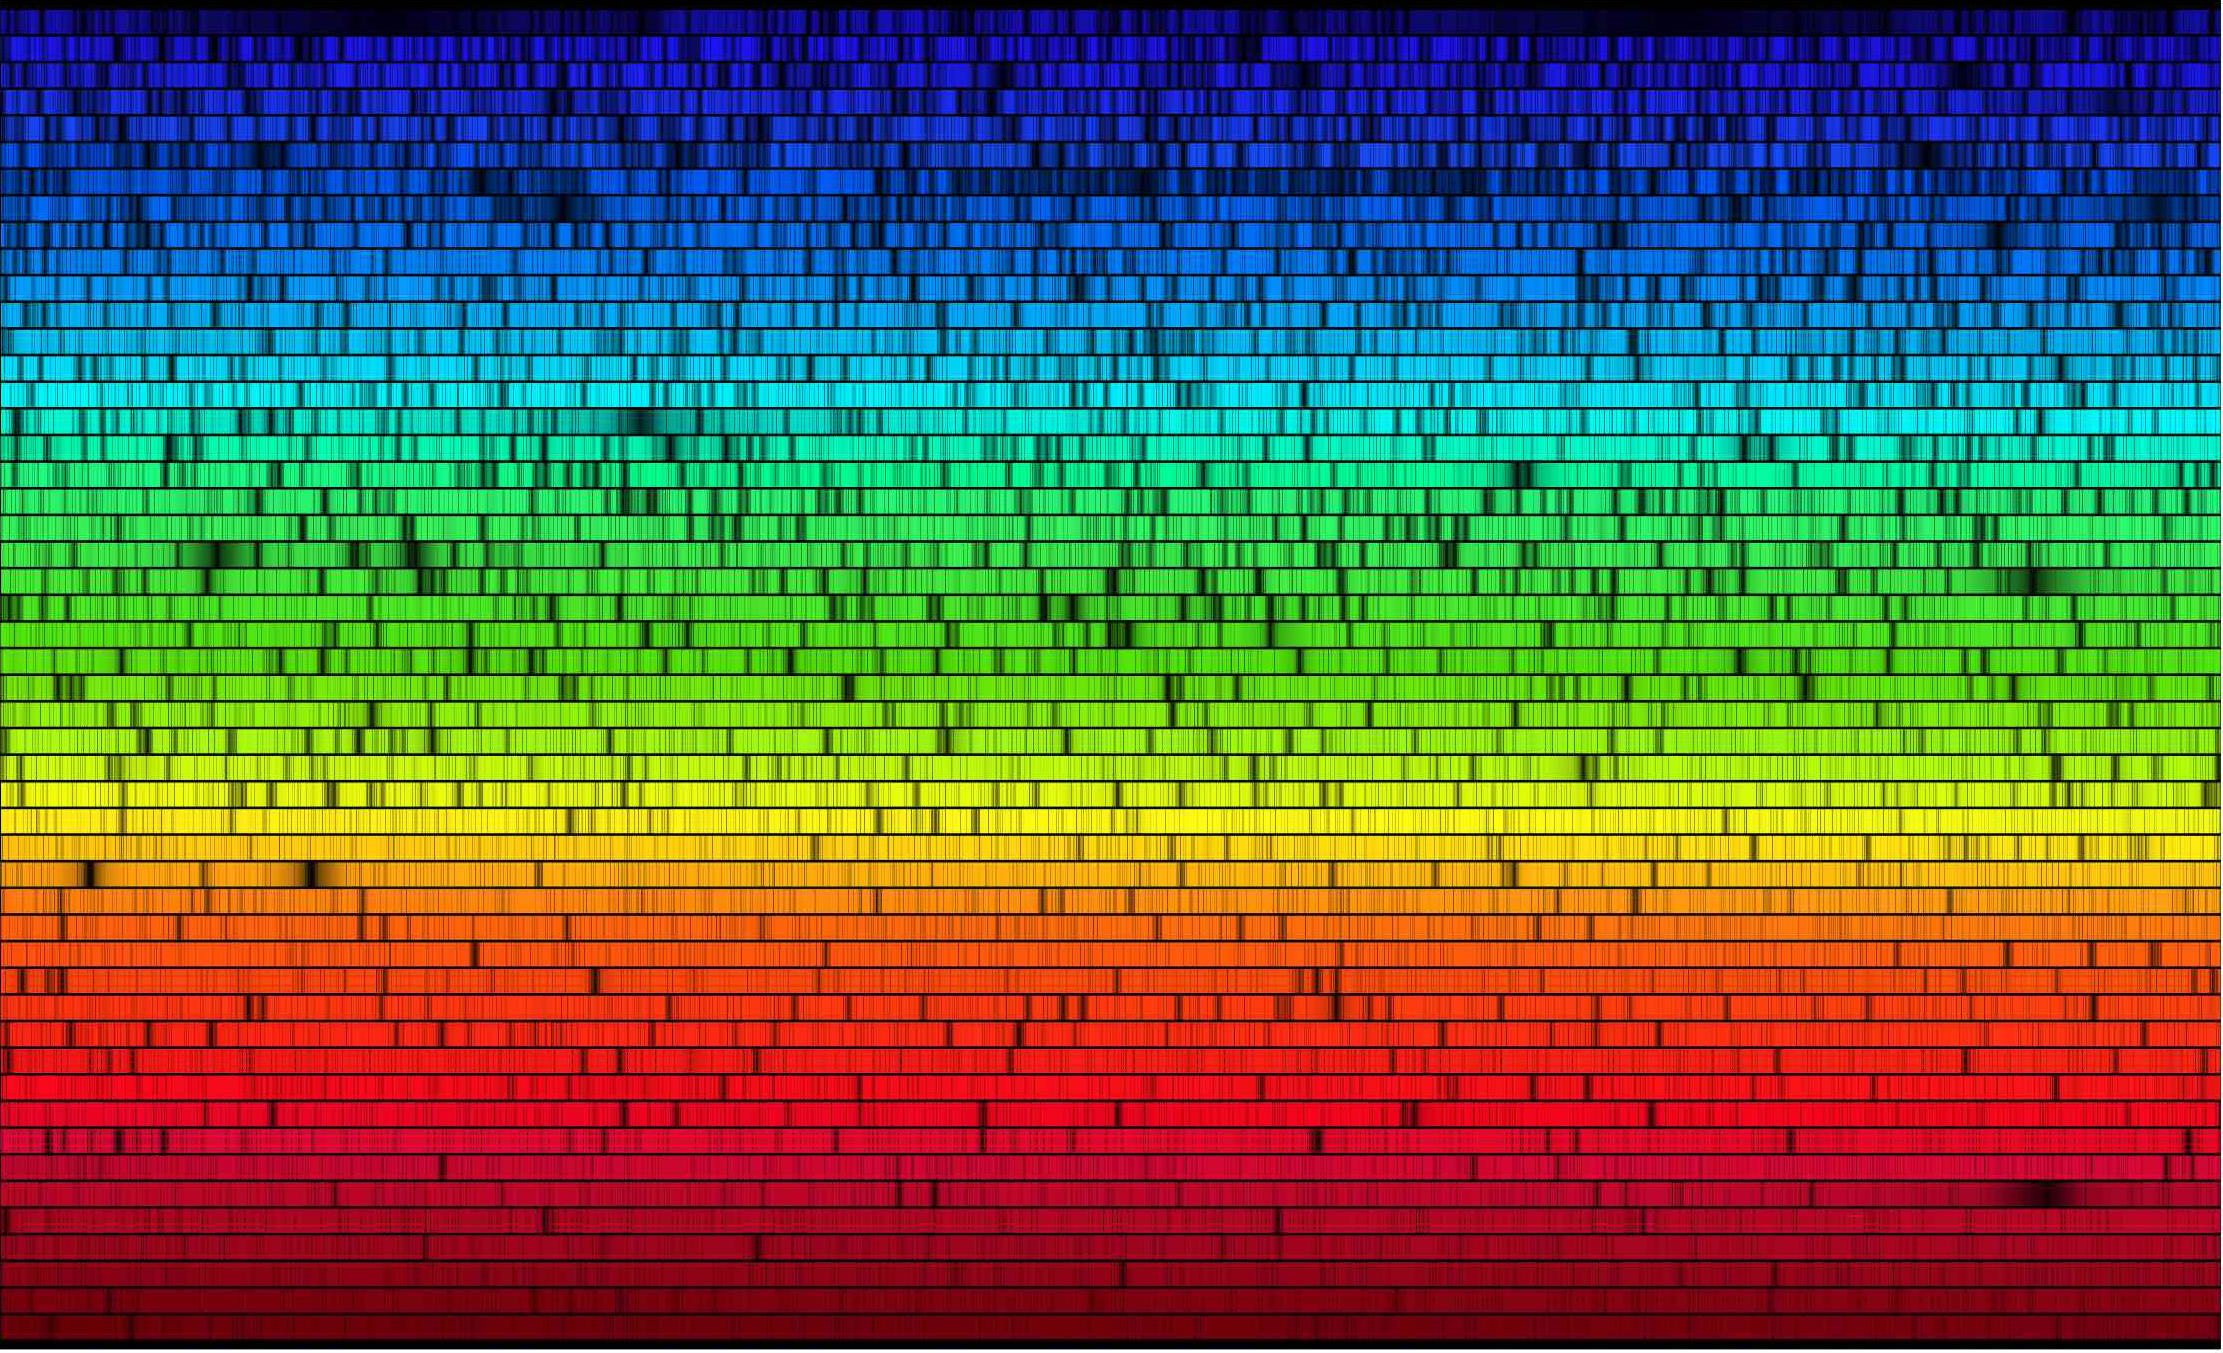
\includegraphics[width=0.45\textwidth]{./images/running/SolarCCD.jpg}
\\
\end{tabular}
\caption{a: A plot of the entire \href{https://commons.wikimedia.org/wiki/File:Solar_Spectrum.png}{solar spectrum}. b: The image below shows the \href{https://solarsystem.nasa.gov/resources/390/the-solar-spectrum/}{solar spectrum} at 392 nm (blue) to 692 nm (red) as observed with the Fourier Transform Spectrograph at Kitt Peak National Observatory in 1981. R. Kurucz }
\end{figure}


\vspace*{\fill}
\fbox{
\parbox{0.9\textwidth}{
\color{blue} Question \addtocounter{question}{1}\thequestion: Describe the main differences between the light which comes from the LED and the sun.  Rather than referring to the various regions of the spectrum by their wavelengths, refer to them using English words, such as $infrared$, $Ultra Violet$, $Red$, and $Green$ etc... you will find which wavelengths match to each color on the internet.  If you were designing a material for a solar cell, what wavelengths would.}
}

\newpage
\subsection{Light inside solar cells}
As you will have seen from when you fist opened the simulation, the solar cells are often made from many layers of different materials.  Some of these materials, are designed to absorb light, some are designed to conduct charge carriers out of the cell.  The simulator has a database of these materials, to look at the database, click on the $Database$ tab, the click on \emph{Material database}.  This should bring up a window as shown in figure \ref{fig:db}, once this is open navigate to the directory $polymers$, and double click on the material $p3ht$, in the new window click on the tab $Absorption$ (see figure \ref{fig:alpha}).  This plot shows how light is absorbed in the material as a function of wavelength.

\begin{figure}[h!]
\centering
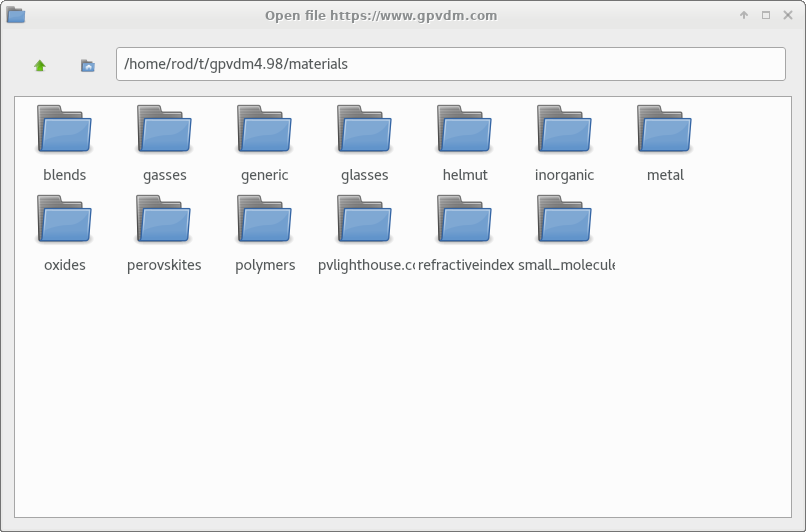
\includegraphics[width=100mm]{./images/running/db.png}
\caption{The materials database}
\label{fig:db}
\end{figure}

\begin{figure}[h!]
\centering
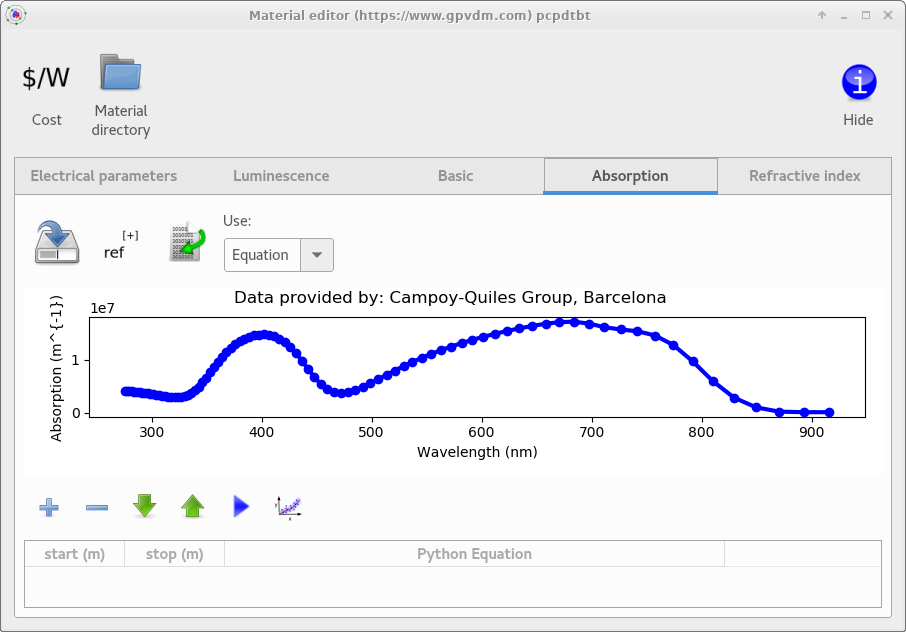
\includegraphics[width=100mm]{./images/running/alpha.png}
\caption{Optical absorption of the light.}
\label{fig:alpha}
\end{figure}

\vspace*{\fill}
\fbox{
\parbox{0.9\textwidth}{
\color{blue} Question \addtocounter{question}{1}\thequestion: What color of light does the polymer $p3ht$ absorb best?  Which material in the $polymers$ directory do you think will absorb the suns light best?}
}


